\section{问题分析与模型假设}

第一问要求计算预热阶段 $1800\,\mathrm{s}$ 内药材的温度与干基含水率，并给出指定时刻和径向位置的结果。药材长 $L=0.25\,\mathrm{m}$、半径 $R=0.02\,\mathrm{m}$，初始温度 $T_0=28\,\celsius$、初始干基含水率 $C_0=2.55\,\kgkg$；物性参数和烘房数据取自题目附录2及附件1\cite{problem}。

圆柱侧面和端面均可发生热、质交换，故采用二维轴对称主模型保留轴向梯度，并用一维径向模型检验中截面结果。取圆柱中心为原点，$r,z$ 分别为径向、轴向坐标；利用对称性计算半域
\begin{equation}
  \Omega=\{(r,z):0\le r\le R,\ 0\le z\le H\},\qquad H=L/2.
  \label{eq:domain}
\end{equation}
轴对称体积元为 $\dd V=2\pi r\,\dd r\,\dd z$，对应半圆柱体积为 $|\Omega|=\pi R^2H$。结果表中的“到药材中心距离”统一解释为\textbf{中截面 $z=0$ 上的径向距离 $r$}。

\subsection{基本假设与适用范围}
\begin{enumerate}
  \item 药材视为连续、均匀、各向同性介质，初始状态均匀；几何尺寸固定，采用题给有效物性参数。
  \item 环境空间上均匀、随时间变化；侧面和两端面均暴露，采用相同的换热、传质系数。
  \item 含水率方程对应空间均匀且固定的干物质体积密度。采用经验闭合 $\Ceq(t)=C_\infty(t)$，将附件1的环境水分数据作为表面传质的等效平衡含水率。
  \item 热量模型考虑导热与对流，水分模型考虑扩散与表面传质；不引入参数不完整的蒸发潜热、吸附等温线及辐射项，其影响作为适用性限制讨论。
\end{enumerate}

\subsection{参数与主要符号}
\begin{center}
\small
\begin{tabular}{lll}
\toprule
符号 & 含义 & 数值或单位\\
\midrule
$T(r,z,t),\ C(r,z,t)$ & 温度、干基含水率 & $\celsius$，$\kgkg$\\
$\Tin(t),\ C_\infty(t)$ & 烘房温度、水分数据 & 附件1，分段线性插值\\
$\rho$ & 密度 & $820\,\mathrm{kg/m^3}$\\
$c_p$ & 比热容 & $2600\,\mathrm{J/(kg\cdot K)}$\\
$k$ & 热导率 & $0.36\,\mathrm{W/(m\cdot K)}$\\
$h$ & 对流换热系数 & $25\,\mathrm{W/(m^2\cdot K)}$\\
$k_m$ & 对流传质系数 & $8\times10^{-7}\,\mathrm{m/s}$\\
$D(C)$ & 有效水分扩散系数 & $7\times10^{-9}\exp(-0.89/C)\,\mathrm{m^2/s}$\\
\bottomrule
\end{tabular}
\end{center}

\clearpage
\section{温度与水分迁移模型}

\subsection{时变环境边界}
在附件1中截取 $0$ 至 $1800\,\mathrm{s}$ 的31个采样点，不作平滑或外推。对任一环境变量 $B\in\{\Tin,C_\infty\}$，在相邻采样时刻 $t_j,t_{j+1}$ 之间取
\begin{equation}
 B(t)=B_j+\frac{t-t_j}{t_{j+1}-t_j}(B_{j+1}-B_j),\qquad t_j\le t\le t_{j+1}.
 \label{eq:ambient}
\end{equation}
由此保留环境温湿度的实际变化，并避免预先设定恒温段。两端时刻的环境温度分别为 $28\,\celsius$ 和 $41.513\,\celsius$，环境水分数据分别为 $0.01963\,\kgkg$ 和 $0.03307\,\kgkg$。

\subsection{控制方程}
根据能量守恒与傅里叶定律，轴对称温度场满足
\begin{equation}
 \rho c_p\frac{\partial T}{\partial t}
 =\frac{1}{r}\frac{\partial}{\partial r}\left(rk\frac{\partial T}{\partial r}\right)
  +\frac{\partial}{\partial z}\left(k\frac{\partial T}{\partial z}\right).
 \label{eq:heat}
\end{equation}
在固定干物质体积密度的假设下，将水分守恒式中的该密度约去，得到
\begin{equation}
 \frac{\partial C}{\partial t}
 =\frac{1}{r}\frac{\partial}{\partial r}\left(rD(C)\frac{\partial C}{\partial r}\right)
  +\frac{\partial}{\partial z}\left(D(C)\frac{\partial C}{\partial z}\right),\quad
 D(C)=7\times10^{-9}\exp\left(-\frac{0.89}{C}\right).
 \label{eq:moisture}
\end{equation}
式\eqref{eq:moisture}必须保留散度形式。由于 $D$ 随 $C$ 变化，展开后有
\begin{equation}
 \nabla\!\cdot[D(C)\nabla C]
 =D(C)\Delta C+D'(C)|\nabla C|^2,\qquad
 D'(C)=\frac{0.89}{C^2}D(C).
 \label{eq:nonlinear}
\end{equation}
直接使用 $D(C)\Delta C$ 会遗漏非线性梯度项。第一问中热物性均为常数，且 $D$ 仅依赖 $C$，因此温度方程与水分方程可以分别求解。

\subsection{初始条件及边界条件}
初始状态为
\begin{equation}
 T(r,z,0)=T_0,\qquad C(r,z,0)=C_0.
 \label{eq:initial}
\end{equation}
在中心轴和中截面分别施加对称条件
\begin{equation}
 \left.\frac{\partial T}{\partial r}\right|_{r=0}
 =\left.\frac{\partial C}{\partial r}\right|_{r=0}=0,\qquad
 \left.\frac{\partial T}{\partial z}\right|_{z=0}
 =\left.\frac{\partial C}{\partial z}\right|_{z=0}=0.
 \label{eq:symmetry}
\end{equation}
令 $\Gamma_e=\{r=R\}\cup\{z=H\}$ 为半域的暴露边界，$\bm n$ 为外法向，$T_s,C_s$ 为表面未知量，则
\begin{equation}
 \begin{aligned}
 -k\nabla T\cdot\bm n&=h(T_s-\Tin),\\
 -D(C_s)\nabla C\cdot\bm n&=k_m(C_s-\Ceq),\qquad \Ceq=C_\infty.
 \end{aligned}
 \label{eq:robin}
\end{equation}
该符号约定下，表面较环境冷时热流向内，表面含水率较高时水分向外迁移。表面状态由式\eqref{eq:robin}求解，而非直接赋成环境值。侧面与端面交界处分别计算两个方向的通量。初始均匀含水率与瞬时失水边界在 $t=0$ 不相容，需保留题设初值并在时间离散中解析启动层。

\clearpage
\section{守恒有限体积离散与非线性求解}

\subsection{轴线、真实表面与交界控制体的统一处理}
采用节点中心有限体积法，节点包含 $r=0,R$ 和 $z=0,H$。内部控制面置于相邻节点中点，物理边界处截断控制体。对控制体 $P$，保留轴对称体积权重
\begin{equation}
 V_P=\pi(r_+^2-r_-^2)(z_+-z_-),\quad
 A_{r,\pm}=2\pi r_\pm(z_+-z_-),\quad
 A_{z,\pm}=\pi(r_+^2-r_-^2).
 \label{eq:volume}
\end{equation}
其中 $r_\pm,z_\pm$ 为控制面坐标。中心轴处 $A_{r,-}=0$，无需在离散式中直接计算 $1/r$；边界半控制体则保留真实表面的状态和交换通量。对侧面与端面交界节点，将两张暴露面的通量同时计入。

记 $N(P)$ 为相邻节点集合，$\mathcal E(P)$ 为控制体暴露面集合，$\ell_{PQ}$ 为节点间距。相邻节点的面扩散系数及热、质传递系数取
\begin{equation}
 D_{PQ}=\frac{2D(C_P)D(C_Q)}{D(C_P)+D(C_Q)},\qquad
 G^T_{PQ}=\frac{kA_{PQ}}{\ell_{PQ}},\quad
 G^C_{PQ}=\frac{D_{PQ}A_{PQ}}{\ell_{PQ}}.
 \label{eq:face}
\end{equation}
于是半离散方程为
\begin{align}
 \rho c_pV_P\dot T_P
 &=\sum_{Q\in N(P)}G^T_{PQ}(T_Q-T_P)
   +\sum_{f\in\mathcal E(P)}hA_f(\Tin-T_P),\label{eq:fvmT}\\
 V_P\dot C_P
 &=\sum_{Q\in N(P)}G^C_{PQ}(C_Q-C_P)
   +\sum_{f\in\mathcal E(P)}k_mA_f(\Ceq-C_P).\label{eq:fvmC}
\end{align}
同一内部面的通量在两个控制体中大小相等、符号相反，全域求和后只剩外边界通量。这使轴线处理、表面交换和整体守恒具有一致的离散表达。

\subsection{非线性 Crank--Nicolson 格式}
将式\eqref{eq:fvmC}写为 $M_C\dot{\bm C}=\bm F(\bm C,t)=L(\bm C)\bm C+\bm b(t)$，其中 $M_C=\operatorname{diag}(V_P)$，$L$ 包含内部扩散项和 Robin 边界的负对角项。时间推进取
\begin{equation}
 M_C\frac{\bm C^{n+1}-\bm C^n}{\Delta t_n}
 =\frac12\left[\bm F(\bm C^{n+1},t_{n+1})+\bm F(\bm C^n,t_n)\right].
 \label{eq:cn}
\end{equation}
为保留新时间层扩散率的非线性，令 $\bm C^{(0)}=\bm C^n$，执行 Picard 迭代
\begin{equation}
 \left[M_C-\frac{\Delta t_n}{2}L(\bm C^{(m)})\right]\bm C^{(m+1)}
 =M_C\bm C^n+\frac{\Delta t_n}{2}
 \left[L(\bm C^n)\bm C^n+\bm b(t_n)+\bm b(t_{n+1})\right].
 \label{eq:picard}
\end{equation}
每次迭代均更新 $D(\bm C^{(m)})$ 及其面调和平均，直至最大含水率增量小于 $2\times10^{-10}$，且新时间层非线性代数方程的残差经 $M_C^{-1}$ 归一化后小于 $2\times10^{-9}\,\kgkg$。温度方程采用相同时间格式，其系数固定，每步直接求解线性方程组。

\clearpage
\subsection{网格加密与初始启动层}
启动后水分梯度首先集中在表面附近，因此采用非均匀网格，径向最后 $1\,\mathrm{mm}$ 区域加密，轴向向端面加密。主计算包含865个径向节点、25个半轴向节点，共21625个节点；径向最大间距为 $0.03125\,\mathrm{mm}$，最小间距约为 $3.90625\,\mu\mathrm{m}$，轴向最小间距约为 $217.014\,\mu\mathrm{m}$。

主时间步长取 $\Delta t=0.5\,\mathrm{s}$。先将 $[0,10^{-4}]\,\mathrm{s}$ 分成两个隐式 Euler 半步，以处理初值与边界条件不相容产生的启动层；随后采用式\eqref{eq:cn}，并按下式限制早期时间步上限：
\begin{equation}
 \Delta t_{\max}(t)=\Delta t\times
 \begin{cases}
  1/5000,&10^{-4}\le t<10^{-3},\\
  1/500,&10^{-3}\le t<10^{-2},\\
  1/50,&10^{-2}\le t<10^{-1},\\
  1/25,&10^{-1}\le t<1,\\
  1/10,&1\le t<10,\\
  1/4,&10\le t<60,\\
  1,&t\ge60.
 \end{cases}
 \label{eq:startup}
\end{equation}
必要时缩短步长以落在分级节点和整数秒输出时刻。该安排是预设分级启动；其精度通过时间步长减半检验，而非由通用局部误差估计器自动保证。

\subsection{求解流程与过程检查}
首先构造控制体体积、面面积和边界类型，并根据式\eqref{eq:ambient}计算各时间层的环境值；随后推进温度场，迭代求解水分场，在每个整数秒提取中截面结果。空间输出点为 $r=0,0.1,\ldots,2.0\,\mathrm{cm}$，其中论文表格取 $0,0.5,1.0,1.5,2.0\,\mathrm{cm}$ 五处。

在计算中同步检查非线性收敛、含水率正值性、温度范围及累计边界通量，不通过裁剪数值强制修正状态。主计算共完成4134个内部时间步，每步 Picard 迭代最多4次，记录的最大非线性残差为 $\NonlinearResidual\,\kgkg$。这些量用于判断离散求解是否完成，不作为模型物理预测精度的证据。

\subsection{精细化处理的作用}
模型的精细化体现在三个方面：有限圆柱几何保留端面交换；非线性扩散率在新时间层内迭代更新；控制体离散统一处理中心轴、表面和端侧交界。边界加密及分级启动进一步针对表面梯度和初始不相容问题分配计算分辨率。其效果由下文的对照计算与守恒检验评价。

\clearpage
\section{第一问计算结果及分析}

\subsection{指定时刻的中截面径向结果}
由二维主模型提取 $T(r,0,t)$ 和 $C(r,0,t)$，按题目指定格式得到表\ref{tab:temperature}和表\ref{tab:moisture}。数值保留四位小数，含水率均为干基量。
\begin{table}[H]
\centering\small
\caption{30分钟内中截面温度（单位：$\celsius$）}\label{tab:temperature}
\begin{tabular}{crrrrr}
\toprule
\multirow{2}{*}{时间 / s} & \multicolumn{5}{c}{到药材中心的距离 / cm}\\
\cmidrule(lr){2-6} & 0 & 0.5 & 1 & 1.5 & 2\\
\midrule
100 & 28.0001 & 28.0003 & 28.0040 & 28.0327 & 28.1801 \\
300 & 28.0408 & 28.0635 & 28.1514 & 28.3681 & 28.8489 \\
600 & 28.4533 & 28.5360 & 28.8039 & 29.3159 & 30.1652 \\
900 & 29.3243 & 29.4583 & 29.8755 & 30.6161 & 31.7304 \\
1200 & 30.5427 & 30.7098 & 31.2223 & 32.1126 & 33.4276 \\
1500 & 31.9957 & 32.1867 & 32.7660 & 33.7463 & 35.1203 \\
1800 & 33.5753 & 33.7720 & 34.3642 & 35.3621 & 36.7856 \\
\bottomrule
\end{tabular}
\end{table}

\begin{table}[H]
\centering\small
\caption{30分钟内中截面干基含水率（单位：$\kgkg$）}\label{tab:moisture}
\begin{tabular}{crrrrr}
\toprule
\multirow{2}{*}{时间 / s} & \multicolumn{5}{c}{到药材中心的距离 / cm}\\
\cmidrule(lr){2-6} & 0 & 0.5 & 1 & 1.5 & 2\\
\midrule
100 & 2.5500 & 2.5500 & 2.5500 & 2.5500 & 2.2471 \\
300 & 2.5500 & 2.5500 & 2.5500 & 2.5492 & 2.0508 \\
600 & 2.5500 & 2.5500 & 2.5500 & 2.5353 & 1.8770 \\
900 & 2.5500 & 2.5500 & 2.5497 & 2.5045 & 1.7547 \\
1200 & 2.5500 & 2.5500 & 2.5482 & 2.4646 & 1.6586 \\
1500 & 2.5500 & 2.5499 & 2.5445 & 2.4206 & 1.5787 \\
1800 & 2.5500 & 2.5497 & 2.5383 & 2.3755 & 1.5102 \\
\bottomrule
\end{tabular}
\end{table}


在 $1800\,\mathrm{s}$ 时，中截面中心与侧面温度分别为 $\FinalCenterT\,\celsius$ 和 $\FinalSurfaceT\,\celsius$，均低于同时刻烘房温度 $41.513\,\celsius$；中心与侧面含水率分别为 $\FinalCenterC\,\kgkg$ 和 $\FinalSurfaceC\,\kgkg$。结果表现为外层升温较快、失水较多，中心水分在这一时间范围内变化很小。表中中心含水率显示为 $2.5500$，仅表示按四位小数舍入后的结果，并非该位置完全没有发生变化。

每隔 $1\,\mathrm{s}$、径向每隔 $0.1\,\mathrm{cm}$ 的完整结果已按题目模板保存于 \texttt{result1.xlsx}，温度与水分浓度各含 $1800\times21$ 个数据值；本文两表均从同一二维主解生成。

\clearpage
\subsection{径向分布与端面影响}
图\ref{fig:profiles}展示七个指定时刻的中截面径向剖面。温度随时间整体升高，表层温度高于中心；水分变化主要集中于外层，且向内部的影响范围随时间扩大。温度与水分的分布差异表明，预热阶段不能用单一均匀状态代替整个径向场。

\begin{figure}[H]
 \centering
 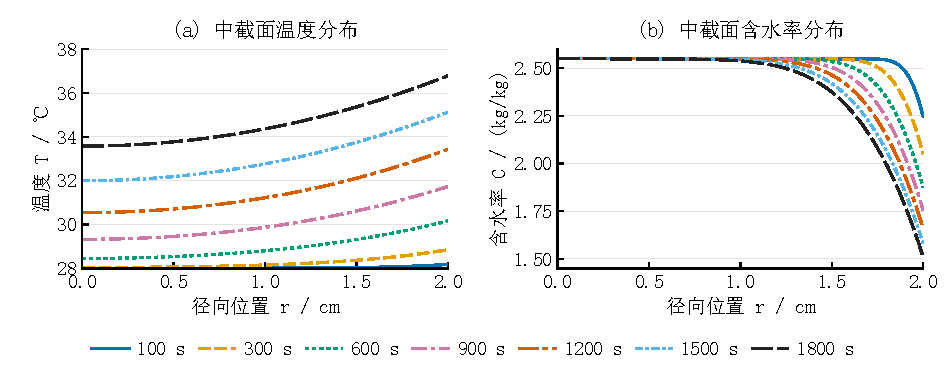
\includegraphics[width=\linewidth]{figures/q1_radial_profiles.pdf}
 \caption{中截面径向剖面：表层先升温，温升逐步向内部传递；含水率下降主要集中于外层。曲线取自二维主解的未舍入快照。}
 \label{fig:profiles}
\end{figure}

为考察端面的影响，建立删除轴向扩散项的一维径向对照，其余物性、初值、径向网格和环境边界与二维主模型一致。定义二维半域体积平均量
\begin{equation}
 \overline u_{\mathrm{2D}}(t)=\frac{2}{R^2H}
 \int_0^H\!\int_0^R u(r,z,t)r\,\dd r\,\dd z,
 \qquad u\in\{T,C\};
 \label{eq:mean}
\end{equation}
一维模型的径向平均为 $\overline u_{\mathrm{1D}}=2R^{-2}\int_0^R u(r,t)r\,\dd r$。两者在 $1800\,\mathrm{s}$ 时的结果见表\ref{tab:means}。
\begin{table}[H]
\centering\small
\caption{$1800\,\mathrm{s}$ 时的体积平均状态对照}\label{tab:means}
\begin{tabular}{lrr}
\toprule
模型 & 平均温度 / $\celsius$ & 平均含水率 / $(\kgkg)$\\
\midrule
二维有限圆柱 & 35.4279 & 2.2748 \\
一维径向对照 & 35.1679 & 2.2936 \\
二维减一维 & 0.2599 & -0.0187 \\
\bottomrule
\end{tabular}
\end{table}


全部指定输出点上，二维中截面与相同径向网格、同步长的一维对照之差很小，但体积平均温度和含水率仍分别相差 $\MeanDeltaT\,\celsius$ 与 $\MeanDeltaC\,\kgkg$。因此，中截面近似一致只支持该位置在30分钟内受到的端面影响很弱，不能据此将端面交换从全域模型中删除。表\ref{tab:means}用于说明端面影响；其四位小数同样是显示格式，不构成全域平均量的严格精度保证。

\clearpage
\section{数值验证与模型评价}

\subsection{中截面网格、时间步长与一维对照}
对温度和含水率分别定义全部输出点的最大绝对差
\begin{equation}
 E_u=\max_{\substack{t=1,\ldots,1800\,\mathrm{s}\\r=0,0.1,\ldots,2.0\,\mathrm{cm}}}
 \left|u_a(r,t)-u_b(r,t)\right|,\qquad u\in\{T,C\}.
 \label{eq:error}
\end{equation}
其中二维数据均取 $z=0$。分别执行同网格一维对照、时间步长减半及径向节点间距减半，结果见表\ref{tab:verification}。
\begin{table}[H]
\centering\small
\caption{全部中截面输出点的最大绝对差}\label{tab:verification}
\begin{tabular}{lrr}
\toprule
比较内容 & 温度 / $\celsius$ & 含水率 / $(\kgkg)$\\
\midrule
二维中截面与同网格一维对照 & $3.74\times10^{-7}$ & $2.21\times10^{-12}$ \\
一维时间步长减半 & $5.35\times10^{-7}$ & $3.88\times10^{-7}$ \\
一维径向网格加密一倍 & $1.13\times10^{-6}$ & $8.38\times10^{-6}$ \\
二维中截面与更细一维参考 & $1.64\times10^{-6}$ & $8.41\times10^{-6}$ \\
\bottomrule
\end{tabular}
\end{table}

时间加密使用一维模型，将主步长从 $0.5\,\mathrm{s}$ 减至 $0.25\,\mathrm{s}$；空间加密在 $0.25\,\mathrm{s}$ 下将径向节点数从865增至1729。最大差支持当前中截面输出的数值收敛性，但网格间差异不是严格解析误差上界，也不保证每个接近舍入分界的单元末位数字均不改变。

\subsection{独立温度参照与整体守恒}
温度方程系数恒定，可另行构造径向特征函数参照。定义热扩散率 $\alpha=k/(\rho c_p)$ 和毕奥数 $\mathrm{Bi}=hR/k$，特征根满足
\begin{equation}
 \lambda_jJ_1(\lambda_j)=\mathrm{Bi}J_0(\lambda_j),\qquad
 a_j=\frac{2J_1(\lambda_j)}{\lambda_j[J_0^2(\lambda_j)+J_1^2(\lambda_j)]}.
 \label{eq:bessel}
\end{equation}
其中 $J_0,J_1$ 为第一类贝塞尔函数。对分段线性的 $\Tin(t)$，可写
\begin{equation}
 \begin{aligned}
 T_{\mathrm{ref}}(r,t)&=\Tin(t)-\sum_{j=1}^{\infty}a_jJ_0(\lambda_jr/R)q_j(t),\\
 q'_j(t)+\frac{\alpha\lambda_j^2}{R^2}q_j(t)&=\Tin'(t),\qquad q_j(0)=0.
 \end{aligned}
 \label{eq:reference}
\end{equation}
在每一线性环境区间内精确推进 $q_j$，并截取512项。256项与512项之差为 $\SeriesDifference\,\celsius$；二维中截面温度与该径向参照的最大差为 $\AnalyticError\,\celsius$。此比较与一维对照相互补充，用于核查中截面热量计算。

对水分定义 $I_C(t)=\int_\Omega C\,\dd V$，对热量定义 $Q_T(t)=\int_\Omega\rho c_p(T-T_0)\,\dd V$。由控制方程及边界条件得到
\begin{align}
 I_C(t)-I_C(0)+\int_0^t\!\int_{\Gamma_e}k_m(C_s-\Ceq)\,\dd A\,\dd\tau&=0,\label{eq:masscheck}\\
 Q_T(t)+\int_0^t\!\int_{\Gamma_e}h(T_s-\Tin)\,\dd A\,\dd\tau&=0.\label{eq:heatcheck}
\end{align}
计算边界积分时采用与时间推进相同的隐式 Euler 或梯形权重。将两式累计残差分别除以 $|\Omega|$ 和 $\rho c_p|\Omega|$，主计算的最大归一化水分、热量平衡残差分别为 $\WaterResidual\,\kgkg$ 和 $\HeatResidual\,\celsius$。这里 $I_C$ 为含水率体积分，若转换为水质量还需乘以定义一致的干物质体积密度。

\subsection{模型适用范围}
有限圆柱几何、含水率依赖的扩散系数以及守恒表面通量，使模型能够描述第一问中径向非均匀的升温与失水过程。现有误差证据主要针对中截面输出：二维端部和端侧交界的全场未认证到四位小数精度，不能将中截面验证结论外推至所有空间位置。

此外，$\Ceq=C_\infty$ 是经验边界闭合。题目没有给出空气水分数据与固体平衡含水率之间的吸附关系，两者单位虽同为 $\kgkg$，分母的物理定义仍可能不同；若取得吸附等温线等资料，应修正此闭合并重新计算。蒸发潜热及尺寸变化未纳入本问模型，也未通过本次计算证明其影响可忽略。由于没有药材内部温湿度实测数据，本文验证的是离散计算的一致性和中截面数值收敛性，不报告实验预测精度。

\begin{thebibliography}{9}
\small
\bibitem{problem} 2026年高教社杯全国大学生数学建模竞赛题目：A题药材的烘干问题[Z]. 2026. 问题1、附录2及附件1.
\end{thebibliography}
